\chapter{Introduction}
\thispagestyle{fancy}
Nowadays, people have smartphones with them all the time. So we thought about why don't we use these to control home appliances of our home. From there we ideated the concept of iHALO (Intelligent Home Assistant\& Lifeline Observer). iHALO as a home automation system is a simple Android app which you can use to control electrical appliances with voice commands, computer vision or just through bots(chat/SMS) . Using the app, you can control all the appliances like TV, fans, light etc. It’s acts as an artificial intelligence which can be controlled using voice command (given by user). You can give the command to switch on or off the devices (like light, fan etc) as well as you can even manipulate them like fan speed, light intensity. Commands are sent via a WiFi module to Arduino. So there is no need for you to get up to switch on or switch off the device while watching a movie or doing some important work.\\
We are also using an AR-augmented reality app to control the appliances and manipulate them. If we want to switch on the electrical appliance we just need to focus the camera and it will start it and using a virtual button, we can switch it off. If we want to know the electricity unit consumed by our appliances along with the cost of units we just need to send a text message to the device (Arduino) through our phone. The Arduino would be connected to the network through a Wi-Fi module which would reply with another text message containing the electricity unit and the total cost consumed by the appliances. This will help the user to get update on the electricity bill and they can decide whether to use the appliances on a regular routine or reduce it usage to save electricity.\\
Our project iHALO, also provides an health monitoring service to the residents in our home specifically could also be used to monitor the health conditions of the old people or patients in our home.
\chapter{Literature Review}
\thispagestyle{fancy}
\begin{enumerate}
	\item  Deepali Javale: Presented the design of home automation and security system using Android ADK, which is based on a standalone embedded system board Android ADK (Accessory Development Kit) at home. This paper put forwards the design of home automation and security system using Android ADK. The design is based on a standalone embedded system board Android ADK(Accessory Development Kit) at home. Home appliances are connected to the ADK and communication is established between the ADK and Android mobile device or tablet. The home appliances are connected to the input/output ports of the embedded system board and their status is passed to the ADK. We would develop an authentication to the system for authorized person to access home appliances. The device with low cost and scalable to less modification to the core is much important. It presents the design and implementation of automation system that can monitor and control home appliances via android phone or tablet.
	\item  Akanksha Singh: presented the paper on how to control home appliances, safety\& security system using GSM technology by using android application through android mobile phone. It can control the appliances even in the absence of android phone by sending a normal sms. The proposed system makes use of existing GSM architecture to control the home appliance. Four different devices are controlled via Android APK. Initially designed APK is installed on Smartphone and messaging is done through sms service, which uses GSM architecture. The sms is received by GSM modem, which is interfaced to Arduino board. In accordance with sms specific device will be turned ON or OFF through relay board.
	\item Prof. R.S. Suryavanshi: discussed a approach in which a model of Home Automation System Using Android and wifi technology, which really offers easy and really much awaited Home Automation Systems (HAS). In this paper, they propose a system, which is very different than the existing system. they implement it with the help of direct Wi-Fi (Wireless Federation), which fits the bill of WLAN 802.11 standard. The main advantage of this system is that it can be implemented with a wider range of not more than 200 meters. It allowscommunicating with a brief and small setup without zap wired connection. This system can be extended for a proper HVAC (Heating, Ventilation and Air Conditioning) system.
	\item Niraj R Chauhan: proposed a system in which if the interrupt is occurred put in the system sends sms to user however user is enable to reply the sms in such a condition associate in nursing intelligent software package can reply sms. In this paper, we describe the design and development of a remote household appliance control system using mobile handset through GSM technology. This system provides ideal solution to the problems caused in situations when a wired connection between a remote appliance/device and the control unit might not be feasible. This paper proposes construction of a micro-controller based automated Home Security System. The door lock is password protected with an LED based resistive screen input panel which operates by detecting difference in light intensity captured by the photo diode which is emitted by surrounding red LEDs and reflected by the finger. This system is aimed at detecting the leakage and sounding an alert so that occupants in the building can maintain optimal ventilation and turn off all electrical appliances or evacuate the vicinity until a redress is made.This paper put forwards the implementation of home automation and security system using Arduino microprocessor and Android smartphone. Home appliances are connected to the microprocessor and communication is established between the Arduino and Android mobile device or tablet via Bluetooth module.
	\item Satish Palaniappan: explained this paper survey of all existing system such as Wi -Fi, GSM, Bluetooth, Zigbee and compare the available feature. Based on all the system surveyed ,is identified as ideal system for home automation with remote access. This paper also gives a comparison of all the above systems described. The systems that have been studied have certain common features. All these systems use a basic underlying communications technology. The advantages and drawbacks of the system derive from this underlying technology. All the systems have a control circuitry that is used to interface with the electrical appliances. There has to be a common command system that will be used to issue commands to the control circuits. The next important feature of the system is the user interface. This determines how the user will interact with the system and extent of control the user exerts over the system. This influences the usability of the system. Most systems also have security features to ensure only authorized access.
	\item  Kouwenhoven SE : He proposed an interface card has been developed to assure communication between the remote user, server, raspberry pi card and the home Appliances. The application has been installed on an android Smartphone, a web server, and a raspberry pi card to control the shutter of windows. Android application on a smartphone issue command to raspberpi card. An interface card has been realized to update signals between the actuator sensors and the raspberry pi card. Cloud-based home appliance monitoring and controlling System.
	Design and implement a home gateway to collect metadata from home appliances and send to the cloud-based data server to store on HDFS (Hadoop Distributed File System), process them using Map Reduce and use to provide a monitoring function to Remote user.
	\item Shih-Pang Tseng et al : proposed Smart House Monitor \& Manager (SHMM), based on the ZigBee, all sensors and actuators are connected by a ZigBee wireless network. They designed a simple smart socket, which can remote control via ZigBee. PC host is used as a data collector and the motion sensing, all sensing data are transferred to the VM in the cloud. The user can use the PC or Android phone to monitor or control through the Internet to power-saving of the house. Arduino microcontroller to receive user commands to execute through an Ethernet shield. Our house network used together both wireless ZigBee and wired X10 technologies
\item  Stanley M, Cheek J: Proposed experiencing an expansion in their population of older people. As people now expect to live longer, they also seek continuing health and well-being throughout their extended old age. Occupational therapists are involved in working towards the attainment of well-being with their older clients. However, their understandings of what well-being for older people entails seems varied, as this examination of the occupational therapy and related gerontological literature reveals.
	\item  Bjørkløf GH, Engedal K, Selbæk G, Helvik AS: Propose the relation between coping and depression in older persons is growing, but research on the concepts and instruments of coping in relation to depression among older persons is scarce and systematic reviews are lacking. With this background, wanted to gain a systematic overview of this field by performing a systematic literature search Jan Reed, Glenda Cook, Sue Childs, and Brendan McCormack: Proposed the paper that reports on some of the findings of a literature review commissioned to explore integrated care for older people recording the aspect of integration of care for older people that was addressed in the paper. Each item was therefore, read and annotated, using a standard data extraction form, according to characteristics such as the form of integration that was addressed the dimension of integration that was addressed the type of publication for research material details about method, design, subjects/participants were recorded, the country of origin, key issues or outcomes that were addressed and key phrases that were identified in the item. From this thematic content analysis, the team identified different strategies, which had been reported on in the literature. These were divided into three levels by the team—macro strategies, which had taken, place at a societal level, mezzo strategies, which had occurred at a service system, level, and micro strategies which had occurred at an individual service.
\end{enumerate}
\chapter{System Analysis}
\thispagestyle{fancy}
In this chapter, we will discuss and analyse about the developing process of iHalo including software requirement specification (SRS) and comparison between existing and proposed system. The functional and non-functional requirements are included in SRS part to provide complete description and overview of system requirement before the developing process is carried out. Besides that, existing vs proposed provides a view of how the proposed system will be more efficient than the existing one.
\section{Existing System}
\thispagestyle{fancy}
Most Advanced home automation systems in existence today require a big and expensive change of infrastructure. This means that it often is not feasible to install a home automation system in an existing building. The Home Automation is a wireless home automation system that is supposed to be implemented in existing home environments, without any changes in the existing infrastructure. The existing infra-red (IR) or Blue-tooth remote controls present in the market are in general appliance specific and the same cannot be used interchangeably. Home appliances are the major sources of energy consumption. Demand management is a key for customizing energy use by managing the lighting, cooling, and heating Systems within residential units. On the other hand, the intelligent operation of activities can also facilitate the optimized management and operation of energy.
\section{Proposed System}
\thispagestyle{fancy}
iHalo is a personal home automation assistant that would help us to control our electrical home appliances with ease, integrated with augmented reality and intended for the common public and also for the visually challenged and speech-impaired persons. This project aims at developing a Home Automation System prototype which mainly focuses on monitoring and controlling household appliances through the Internet interface module and a software communication module. The Hardware interface module consists of: Arduino 101, Wi-Fi module and relays. The central device is the microprocessor that connects to the Wi-Fi module and receives orders to monitor and control the appliances. The communication between the application and microprocessor is handled by the server, thus managing the users and the appliances. The software communication module uses an Android application as the frontend, which serves as an interface to the user to communicate with the microprocessor. It presents a list of devices with which the user can interact.\\
The system offers switching functionalities to control the appliances connected to the system, which includes Lights, Fans, Air-conditioners and various other appliances connected to the system. In India, the alternating current supplied to our homes is of 230V. Arduino Board is not capable of withstanding such high Voltages. Thus, Relays are used to convert this high voltage to low voltage i.e. less than 5V. The relay switches have capability to carry a maximum load of 10A at 240V. To enable connectivity with the microcontroller Wi-Fi module is used.\\
Blind people can control electrical appliances with the help of simple voice commands like “iHalo turn on the Fan” that is by using android app you can give the command to control your room electrical appliances. It can also be used for dumb people with the help of an AR(Augmented Reality) to control the appliances and manipulate them. If we want to switch on the electrical appliance we just need to focus the camera and it will start it using a virtual button and we can switch it off.\\
iHalo provides Internet connectivity, which allows Internet access and control from the Android Application effectively and efficiently. The Android application is a user friendly interface, which enables the user to view the status of applications at home and control it as per his/her requirement.
\section{Project Modules}
\thispagestyle{fancy}
The modules in the project are :
\begin{enumerate}
	\item Smart Home Assistant module: To control electrical home appliances
	\item  Health monitoring module: To monitor the health conditions of the old people.
\end{enumerate}

\chapter{Requirement Specifications}
\thispagestyle{fancy}
This section describes the software and hardware requirements of the system.
\section{Hardware Requirements}
iHALO Home Assistance
\begin{itemize}
	\item  LDR (Light Dependent Resistor): We put this device inside an Energy Meter which is entirely encapsulated with black tape to eliminate sunlight interference. The rate at which the light blinks in the energy meter is used to determine the power consumption.
	\item  Wi-Fi Module: Here we use ESP8266 Wi-Fi module to connect our Arduino to the internet and make connection with IoT Cloud like Thingspeak, Blynk.
	\item  Arduino 101: The Arduino/Genuino 101 is a learning and development board which contains the Intel® Curie™ Module, designed to integrate the core's low power consumption and high performance with the Arduino's ease-of-use.
	\item  4 channel 12V 10A relay control board module: A relay is an electromagnetic switch operated by a relatively small electric current that can turn on or off a much larger electric current. The heart of a relay is an electromagnet (a coil of wire that becomes a temporary magnet when electricity flows through it). You can think of a relay as a kind of electric lever: switch it on with a tiny current and it switches on ("leverages") another appliance using a much bigger current.
	\item  Jumper Wires: A jump wire is an electrical wire or group of them in a cable with a connector or pin at each end, which is normally used to interconnect the components of a breadboard or other prototype or test circuit, internally or with other equipment or components, without soldering .
\end{itemize}

iHALO Band
\begin{itemize}
	\item  Infineon DPS310: The barometric pressure sensors DPS310 offers excellent pressure noise performance and high stability with temperature.
	\item  Arduino Nano: The Arduino Nano is a small, complete, and breadboard-friendly board based on the ATmega328; offers the same connectivity and specs of the UNO board in a smaller form factor.
	\item  Wifi module : Here we use ESP8266 WiFi module to connect our arduino to the internet and make connection with IoT Cloud like Thingspeak, Blynk.
	\item 4v LiPo Battery: For powering up, Arduino Board.
	\item  Jumper Wires: A jump wire is an electrical wire or group of them in a cable with a connector or pin at each end, which is normally used to interconnect the components of a breadboard or other prototype or test circuit, internally or with other equipment or components, without soldering.
	\newpage
\end{itemize}


\section{Software Requirements}
\begin{itemize}
	\item  Operating system: Android OS v4.4 and above to execute our iHALO app.
	\item  Arduino IDE: The Arduino Board is programmed using the Arduino Software (IDE), the Integrated Development Environment.
	\item  Android Studio: Android Studio is the official integrated development environment (IDE) for Google's Android operating system, built on JetBrains IntelliJ IDEA software and designed specifically for Android development. It is a replacement for the Eclipse Android Development Tools (ADT) as primary IDE for native Android application development.
	\item  IoT Platform: Blynk is a Platform with iOS and Android apps to control Arduino, Raspberry Pi and the likes over the Internet. It's a digital dashboard where you can build a graphic interface for your project by simply dragging and dropping widgets.
	\item  AR development Tools: Unity with Vuforia is a software platform for creating Augmented Reality apps. Developers can easily add advanced computer vision functionality to any application, allowing it to recognize images and objects, and interact with spaces in the real world.
	\item  Programming Language: Arduino Board is coded in C language. Android app may be developed in Java or Kotlin language.
\end{itemize}
\chapter{System Design}
\thispagestyle{fancy}
\section{Use Case Diagram}

\begin{figure}[H]
	
	\centering
	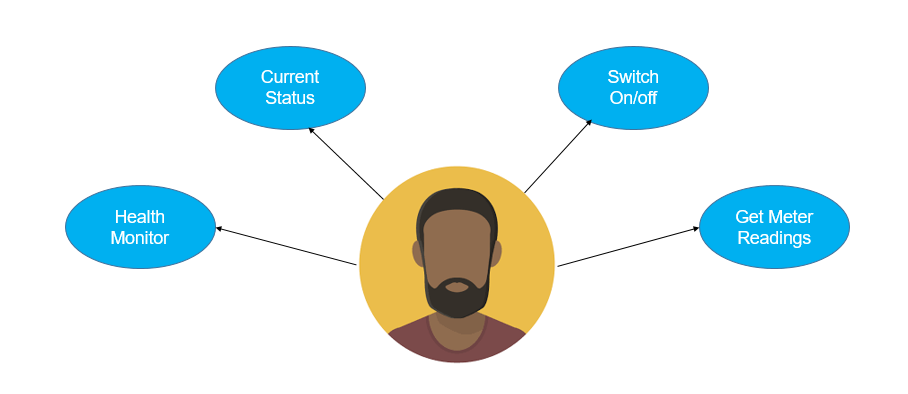
\includegraphics[width=\linewidth,height=7cm] {./images/p1.png}
	\caption{Use Case Diagrams}
	\label{manual}
\end{figure}
A use case diagram is a graphic depiction of the interactions among the elements of a system. A use case is a methodology used in system analysis to identify, clarity and organize system requirements. Here the user can monitor his health, current status of home appliances, make devices switch on or off, and even get current meter readings.
\section{Data Flow Diagram}
\begin{figure}[H]
	
	\centering
	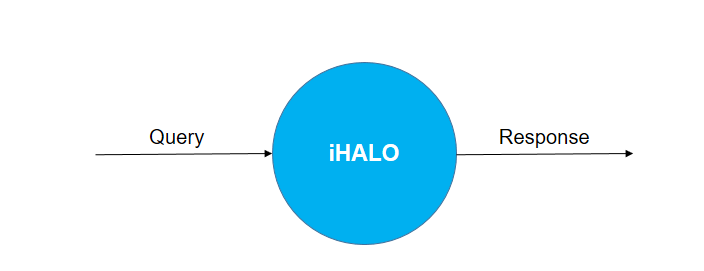
\includegraphics[width=\linewidth,height=7cm] {./images/p2.png}
	\caption{Data Flow Diagram}
	\label{manual}
\end{figure}

This is the level 0 DFD also known as context level diagram where the whole system is considered as a single unit. The users pass a query in form voice commands, computer vision or through just text. Our system then processes this query, to perform necessary action to be performed. Response may be in form of switching on or off the home appliances or get the status of various devices (including Band).
\begin{figure}[H]
	
	\centering
	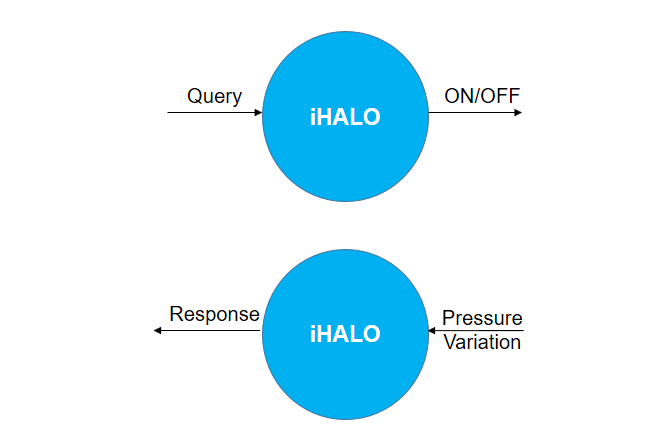
\includegraphics[width=\linewidth,height=8cm] {./images/p3.png}
	\caption{Level DFD}
	\label{manual}
\end{figure}

The level 1 DFD describes about the procedures/actions done by the user \& the system. Our system is divided into two sub systems. One subsystem is, iHalo as a Home assistant where you can give the command to switch on or off the devices (like light, fan etc.) as well as you can even manipulate them like fan speed, light intensity.\\
Another subsystem is, iHalo as Health monitor provides a health monitoring service to the residents in our home specifically could also be used to monitor the health conditions of the old people/patients in our home. Here the input is pressure variations and response is provided by iHalo after analysing the input.\\
Our band will be able to analyse/detect :
\begin{figure}[H]
	
	\centering
	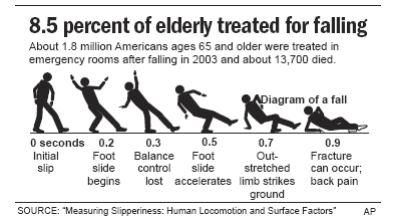
\includegraphics[width=\linewidth,height=10cm] {./images/p4.png}

	\label{manual}
\end{figure}
\textbf{Fall} - Big drop and constant altitude states that patient has fallen and can't get up.\\
Studies show that the biggest issue with elders are of them losing balance and falling down. Often patients are helpless and it's only after sometime that help comes. This could be easily avoided with the Health Band by the detection of a sudden drop in pressure. Once detected a message is automatically sent to relatives, for aid preventing the injury to worsen.\\
\begin{figure}[H]
	
	\centering
	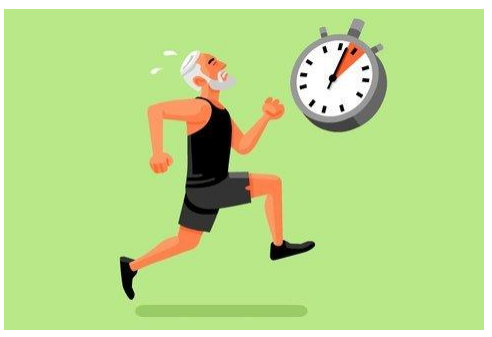
\includegraphics[width=\linewidth,height=8cm] {./images/p5.png}

	\label{manual}
\end{figure}\\

\textbf{Exercise} - Wave like motion depicting a step, this was generated by walking around the room with the band tied on my foot.\\
For old people it can be rather hard to get them to exercise, or go for a walk even though this will keep them fit and healthy. We figured that a way to motivate them could be by showing them the number of steps taken or in how much time they have walked for, so that they have something to push them to exercise. Once the Health Band detects a "wave" motion it deducts that the patient has begun his/her exercise. Crest to crest or trough to trough marks one cycle. As steps are taken the number of cycles are generated and then displayed.\\
\textbf{Fever} - Normal body temperature is around 37 degrees Celsius\\
This one is pretty straight forward the sensor also gives the temperature. The band being in contact with the arm gives the live temperature of the patient. Any spikes or drops will be alerted again automatically via message to relatives.\\
\textbf{State} - No change in altitude for a period of time could suggest that the patient is asleep.\\
Tells the relatives the live state of the patient. For example, if the Health Band detects not much changes of pressure the patient could be sleeping.
\section{Block Diagram}
\begin{figure}[H]
	
	\centering
	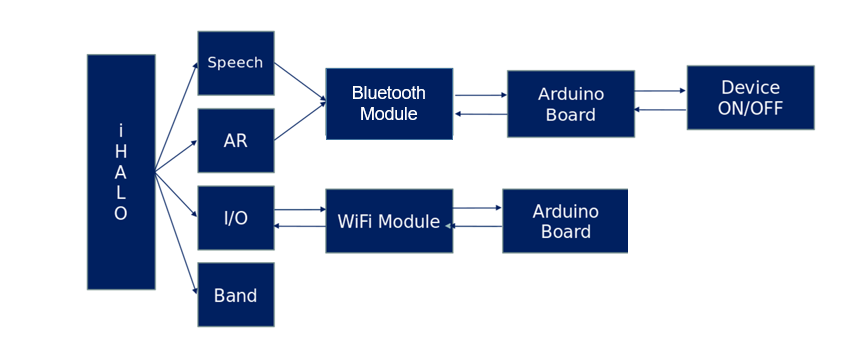
\includegraphics[width=\linewidth,height=10cm] {./images/p6.png}
	\caption{Block Diagram of iHALO}
	\label{manual}
\end{figure}
\textbf{The Digital Energy Meter}\\
In the energy meter, a LDR (Light Dependent Resistor) is used to take the blink speed according to the load. The blink per second value is fed into the Arduino for further calculation units and the value of energy consumed. These are sent to the user via the GSM module. The user can then comprehend which appliance is consuming more power and take action accordingly.
\textbf{The AR Virtual Assistant}\\
The AR Virtual Assistant works using an android app which is installed on the user’s android phone. The android app is connected to the Arduino 101 via Wi-Fi which is in turn connected to the relay and hence the electrical appliances. If we want to switch on the electrical appliance we just need to focus the camera and it will start it and using a virtual button, we can switch it off.\\
\textbf{The Voice Assistant}\\
The Voice Assistant of iHALO works using an android app which is installed on the user’s android phone. The user activates the agent using the wake up command.\\
The android app is connected to the Arduino 101 via Wi-Fi which is in turn connected to the relay and hence the electrical appliances.\\
The flow of signals is as follows:\\
 1. Voice Input/AR Interface\\
 2. Processing on Sensor\\
 3. Sending encrypted data to Arduino via Wi-Fi Module.\\
 4. Processing on Arduino 101\\
 5. Digital signals to relay\\
 6. Operate the Device According to the Digital Data.\\
Pins connections:\\
• Pin 8 -- $>$ Pulse In [Digital Input]\\
• Pin 6 -- $>$ IN1 -- $>$ Device1 Output\\
• Pin 4 -- $>$ IN2 -- $>$ Device2 Output\\
• Pin 5 -- $>$ IN3 -- $>$ Device3\\
Connections of Energy meter:\\
1. Connect the meter to the supply.\\
2. Cover the energy meter with a black tape, preventing the LDR inside the energy meter from outside light.\\
3. Connect the neutral wire directly to the loads and the phase wire to the relay.\\
4. Take the wires from the LDR outside the meter to the counter circuit.\\
5. Now take the output from the counter circuit to the assigned pin 8 pulse pin.\\
6. Connect the TX, RX pin of the Arduino 101 to RX, TX pin of the GSM module.\\
7. Now power up the boards after burning the code.\\
\section{Sequence Diagram}
\begin{figure}[H]
	
	\centering
	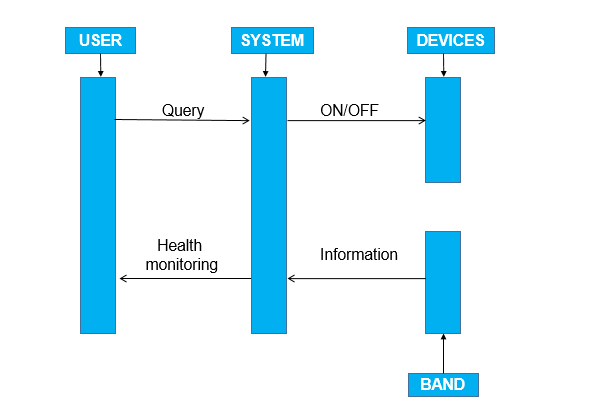
\includegraphics[width=\linewidth,height=8cm] {./images/p7.png}
	\caption{Sequence Diagram}
	\label{manual}
\end{figure}
It is an interaction diagram that shows how object operate with one another and in what order. It is a construct of message sequence chart. It shows the object interaction arranged in time sequence.\\
Sequence diagrams are a popular dynamic modelling solutions. Dynamic modelling focuses on the interaction occurring within the system. Sequence diagram specially focus on the lifelines of an object and how they communicate with other object to perform a function before lifeline ends. The main three objects of our project are user, system and devices. A sequence diagram shows object interactions arranged in time sequence. It depicts the objects and classes involved in scenario and the sequence of messages exchanged between the objects needed to carry out the functionality of the scenario. Sequence diagrams are typically associated with use case realizations in the logical view of the system under development. Sequence diagrams are sometimes called event diagrams or event scenarios. The user interacts with system by passing query. The system processes the query, and take an action to switch the device on or off. iHALO band monitors the health condition of users. According to the pressure variations from the body, response is provided by iHalo after analysing the input.
\chapter{System Testing}
\thispagestyle{fancy}
\section{ Testing, Training and Documentation}
Testing is the stage of implementing, which is aimed at earning system running accurately and efficiently. The purpose of the system testing is to identify and correct errors in the new system. The performance factors like turnaround time, back up, file protection and human factors are some of the performance criteria for system testing. A system is tested for online response, volume of transactions, recovery from failure and usability.
Effective testing early in the process translates directly into long-term costsavings from a reduced number of errors. Back up files are need when the system is failure or down. The usability test verifies the user-friendly nature of the system. Accurate and complete documentation is necessary for the user-friendly nature of the system.\\
System testing is designed to uncover weaknesses that are not found in the earlier tests. This includes forced system failure and validation of the total system, as its users in the operational environment will implement it. Generally it begins with low volume of transactions based on live data. The volume is increased until the maximum level for each transaction type is reached. The total system is tested for recovery and fallback after various major failures to ensure that no data are lost during the emergency. All this is done with the old system still in operation. After the candidate system passes the test, the old system is discontinued.\\
System testing involves unit testing, integration testing, acceptance testing.Careful planning and scheduling are required to ensure that modules will be available for integration into the evolving software product when needed. A test plan has the following steps :\\
1. Prepare test plan\\
2. Specify conditions for user acceptance testing\\
3. Prepare test data for program testing\\
4. Prepare test data for transaction path testing.\\
5. Plan user training\\
6. Compile/assemble programs\\
7. Prepare job performance aids.\\
System testing is the stage of implementation that is aimed at ensuring that the system works accurately and efficiently before live operation commences. The system on a whole was tested for the following:\\
1. Validation of inputs\\
2. Referential integrity test\\
3. Sequential tests\\
4. Consistency of the application\\
System testing, asks a logical assumption that if all the parts of the system are correct, the system will be successfully achieved. The objective of testing is to discover errors. To fulfill these objectives a series of tests were planned and executed. The logical design and the physical design should be thoroughly and continually examined on paper to ensure that they will work when implementation should be a confirmation that all is correct and an opportunity to show the users that the system.\\
\newpage
\section{ Unit Testing}
Here, each individual program was tested using the test data. The outputs as per the requirements were found satisfactory. Thus it was possible to conclude that every program in the software was functionally correct. The interrelated modules were also tested in an exhaustive that will make the whole software work properly.Module interface is tested to ensure that information properly flows into and put of the program under test.This test focuses verification effort on the smallest unit of software design, the module. Here, the module interfaces, local data structure, boundary conditions, and all independent paths and last but not the least, all error handling paths were verified by in putting false data. Tests of data flow across each module interface of this software were done before any other test was initiated.\\
A unit testing focuses on the verification effort on the smallest unit of the software design. Using the unit test plan, prepared in the design phase of the system, important control paths had tested to uncover the errors within these modules. This testing was carried out doing the coding itself. In this testing step, each module is going to be working satisfactorily as the expected output from the module.\\
\section{ Integrated Testing}
The individual programs are combined together to form modules. Integrated tests were performed on each of the modules and again the validity was checked. After that, all modules were brought under a single module and the integrity test was found to be successful. This system was validated in such a way that even the slightest deviation in inputting the data will invoke error messages and provide guidelines regarding the input. Before the software is being released, the developers to do testing by implementing the commercial security package for security. This ensures that the software works properly.\\
These tests can also be performed\\
1.Top down integration\\
2.Bottom up integration\\
It is systematic technical for constructing the program structure while at the same time conducting test to uncover errors associated with the interface. The objective is to take unit tested module and build the program structure that has been detected by design. All modules are combined in this testing step, and the entire program is tested as a whole. If a set of errors are encountered correction is difficult because the isolation of causes is complicated by vastness of the entire program. Using integrated system test plan prepared in the design phase of the system developed as a guide, he integration was carried up.\\
\section{ Validation Testing}
Validation testing is done to ensure complete assembly of the error-free software. Validation can be termed successful only if it functions in manner that is reasonably expected by the customer. Under validation is alpha and beta testing. Alpha testing iswhere the end user tests the system rather than the developer, but in a controlled environment. The software is used on a natural setting with the developer monitoring the user using the system. The developer records the errors and usage problems encountered by the user. The sales person conducts beta testing at one more sites. The developer is not present during these tests. Hence, beta test can be said as the live application of the software on an environment that cannot be controlled by the developer. The sales person takes down the problems encountered during beta testing and reports these to the developer at regular intervals. The developer makes suitable modifications to the software henceforth. The first step in system testing is to develop a plan that tests all the aspects of the system. Completeness, correctness, reliability and maintainability of the software are to be tested for the best quality assurance-an assurance that the system meets the specification and requirements for its intended user and performance. System testing is most useful practical process of executing a program with explicit intention of finding errors that makes the program fail. The following phases were developed.
\section{ Module Testing}
Each individual programs module is tested for any possible errors. They were also tested for specifications, i.e. to see whether they are working as per what the program should do and how it should perform under various conditions.
\section{ Concurrence Testing}
Since the system is a multi-user it was tested for concurrence problems. The system worked perfectly since the table locking and other security measures were taken with care by the database itself.

\section{Display Testing}
The display procedures were tested since the displayed is of much importance. The data was input in the different modules and it was checked whether the information is properly displayed in the other dependent modules. The consistency of the display and attractiveness of the display were also tested. The following tests were also conducted over the system developed:\\
Integration:\\
 These test the integration between browsers and servers, applications and data, hardware and software.\\
Usability:\\
 These test the overall usability of a web page or a web application, including appearance clarity and navigation.\\
Security:\\
 These test the adequacy and correctness of security controls including access control and authorizations.\\
Performance:\\
 These test the performance of the web applications under load.
Verification of code: this validate that the code used in building the web application has been used in a correct manner.\\
Comments and suggestions from the observations during the test run were later considered. Special care was given to user interface comments. The list of possible values, the attractiveness and user-friendliness of the software was well appreciated.A well-designed system, if not operated and used properly could fail.\\
Training the users is important, as if not done well enough could prevent the successful implementation of an information system. Through the systems development life cycle the user has been involved. By this stage the analyst should possess an accurate idea of the users they need to be trained. They must know what their roles will be, howthey can use the system and what the system will do and will not do. Both system operators and users need training. During their training, they need to be given a trouble-shooting list that identifies possible problems and identifies remedies for the problem. They should be advised of the common malfunctions that may arise and how to solve them.\\
Once the implementation plan is decided, it is essential that the user of the system is made familiar and comfortable with the environment. Education involves right atmosphere\& motivating the user. A documentation providing the whole operations of the system is being developed.\\
The system is developed in such a way that the user can work with it in a well consistent way. The system is developed user friendly so that the user can work the system from the tips given in the application itself. Useful tips and guidance is given inside the application itself to help the user. Users have to be made aware that what can be achieved with the new system and how it increases the performance of the system.

\chapter{Prototype}
\thispagestyle{fancy}
\begin{figure}[H]
	
	\centering
	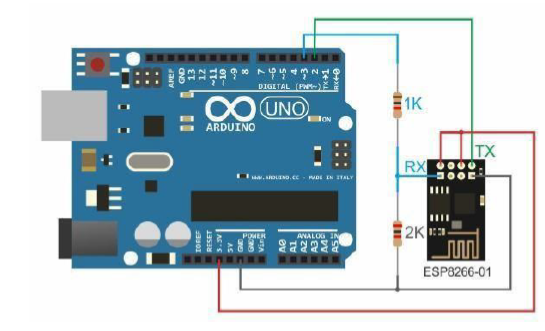
\includegraphics[width=\linewidth,height=7cm] {./images/p9.png}
	\caption{Prototype Schematic}
	\label{manual}
\end{figure}

We implemented a cut down version of iHALO, to check whether our proposed system can be made into reality. For this we used an Arduino Board, ESP8266 Wi-Fi module, a LED and resistor (300 ohm). Blynk platform came handy for prototyping. Our objective was to make LED glow when we switch on the button on the Blynk app. The Blynk app sends the request to increase the voltage in D13 pin. As a result, our LED glows. The experiment was success and the output was verified.
\chapter{Appendices}

\thispagestyle{fancy}
\section{Appendix-I: Arduino code}
\begin{lstlisting}[language=Arduino] 
String voice;
int ihalo = 9;
int router = 10;
int light = 11;
int fan = 12;
void ihaloOn(){
	digitalWrite(ihalo,LOW);
}
void ihaloOff(){
	digitalWrite(ihalo,HIGH);
}
void routerOn(){
	digitalWrite(router,LOW);
}
void routerOff(){
	digitalWrite(router, HIGH);
}
void lightOn(){
	digitalWrite(light,LOW);
}
void lightOff(){
	digitalWrite(light,HIGH);
}
void fanOn(){
	digitalWrite(fan,LOW);
}
void fanOff(){
	digitalWrite (fan, HIGH);
}
void allon() {
	digitalWrite(ihalo,LOW);
	digitalWrite(router,LOW);
	digitalWrite(light,LOW);
	digitalWrite(fan,LOW);
}
void alloff(){
	digitalWrite(ihalo,HIGH);
	digitalWrite(router,HIGH);
	digitalWrite(light,HIGH);
	digitalWrite(fan,HIGH);
}
void setup(){
Serial.begin(9600);

//define output pins
pinMode(ihalo,OUTPUT);
pinMode(router,OUTPUT);
pinMode(light,OUTPUT);
pinMode(fan,OUTPUT);

// set all devices as 'OFF' on Initialisation
digitalWrite(ihalo,HIGH);
digitalWrite(router,HIGH);
digitalWrite(light,HIGH);
digitalWrite(fan,HIGH);
}
void loop(){   // read commands sent using bluetooth
while(Serial.available()) {
	delay(10);
	char c=Serial.read();
	if(c=='\#')
	{break; }
	voice += c; }

if (voice.length() > 0) {
	Serial.println(voice);
	if (voice == "on" || voice == "all")
	{
		allon() ;
	}
	else if (voice == "of" || voice=="off")
	{
		alloff() ;
	}
	else if(voice =="ihalo on" || voice =="hi hello"){
		ihaloOn();
	}
	else if(voice =="hi hello off" || voice =="log out" ){
		ihaloOff();
	}
	else if(voice =="router" || voice =="router on"){
		routerOn();
	}
else if( voice =="router off" || voice =="router of"){
routerOff();
}
else if(voice =="light" || voice =="light on"){
lightOn();
}
else if(voice =="light off" || voice =="light of"){
lightOff();
}
else if(voice =="fan" || voice =="fan on"){
fanOn();
}
else if(voice =="fan off" || voice =="fan of"){
fanOff();
}
voice="";   //make string empty
}}
\end{lstlisting}
\section{Appendix-II: Development \& Testing}
\begin{figure}[H]
	
	\centering
	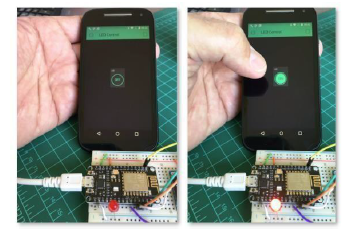
\includegraphics[width=\linewidth,height=7cm] {./images/p10.png}
	\caption{Home Automation Prototype}
	\label{manual}
\end{figure}\\

\begin{figure}[H]
	
	\centering
	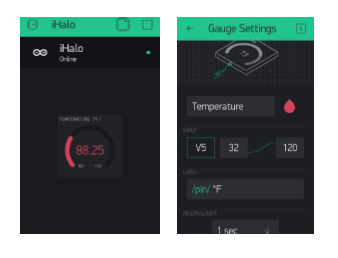
\includegraphics[width=8cm,height=7cm] {./images/p11.png}
	\caption{iHALO Band App}
	\label{manual}
\end{figure}\\

\begin{figure}[H]
	
	\centering
	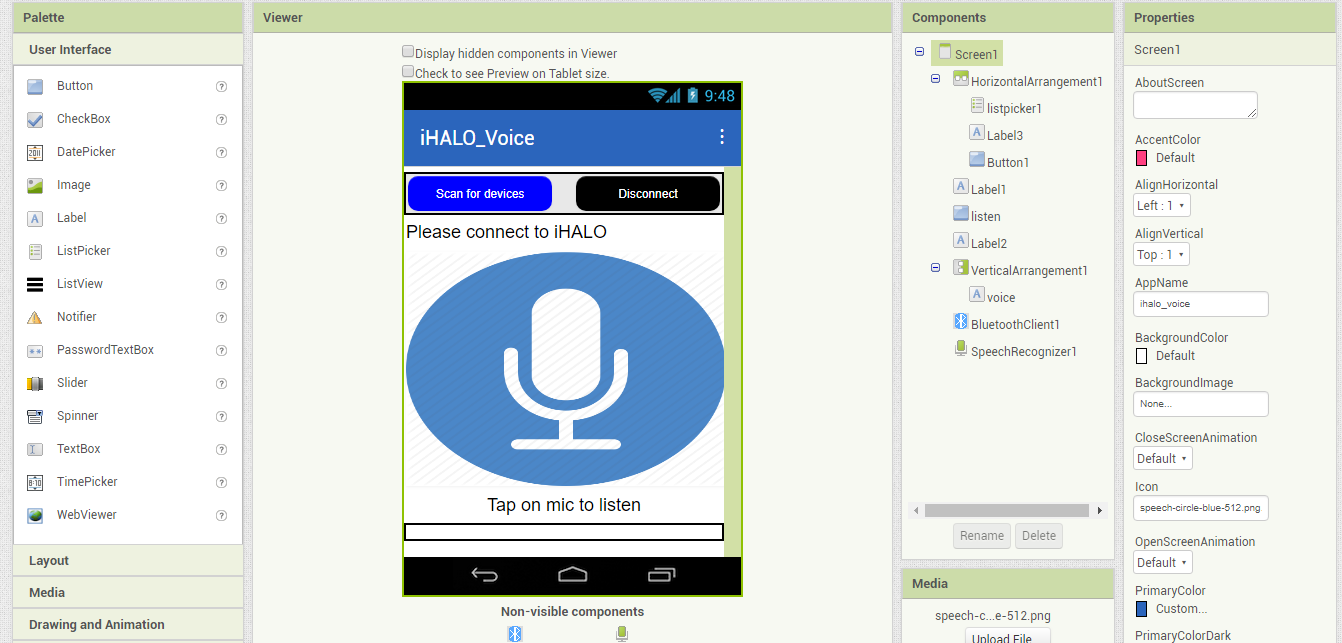
\includegraphics[width=\linewidth,height=10cm] {./images/p13.png}
	\caption{UI Design of iHALO Voice}
	\label{manual}
\end{figure}

\begin{figure}[H]
	
	\centering
	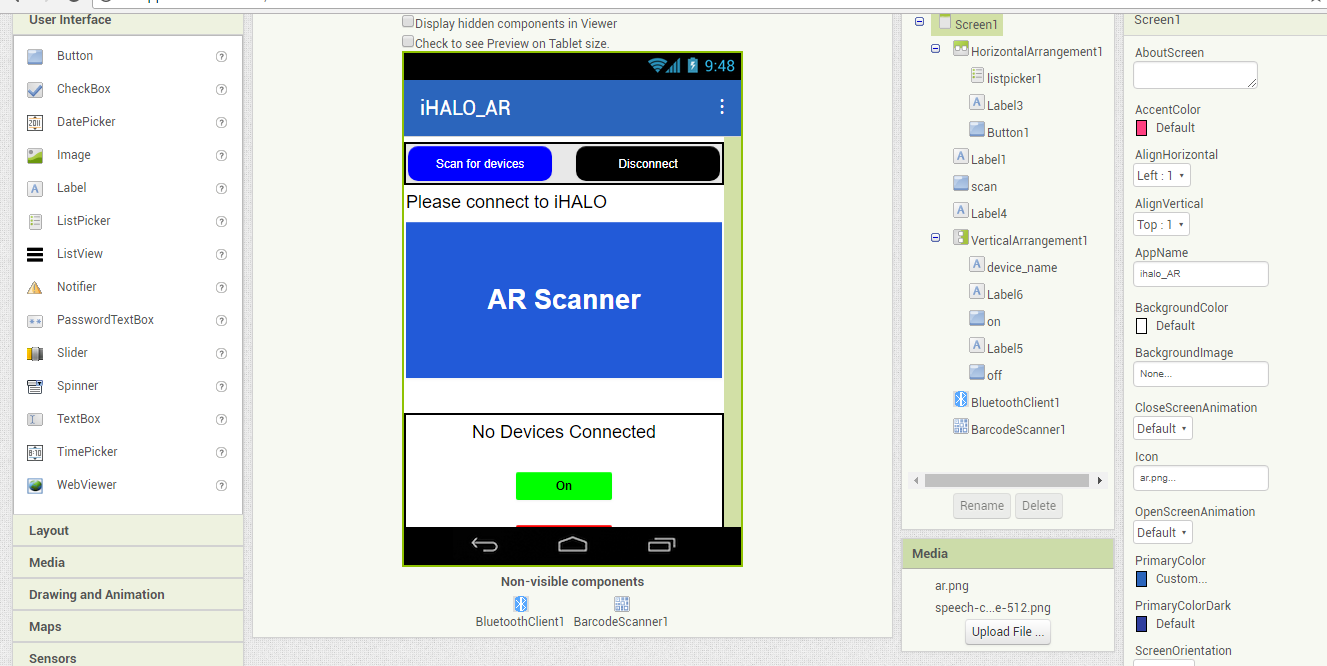
\includegraphics[width=\linewidth,height=10cm] {./images/p14.png}
	\caption{UI Design of iHALO AR}
	\label{manual}
\end{figure}\\

\begin{figure}[H]
	
	\centering
	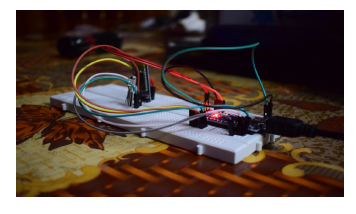
\includegraphics[width=\linewidth,height=8cm] {./images/p15.png}
	\caption{Experimental Setup-I}
	\label{manual}
\end{figure}

\begin{figure}[H]
	
	\centering
	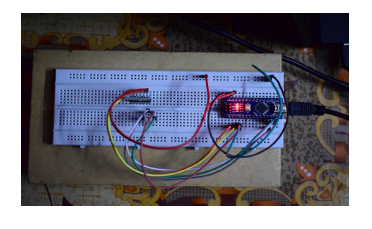
\includegraphics[width=\linewidth,height=8cm] {./images/p16.png}
	\caption{Experimental Setup-II}
	\label{manual}
\end{figure}\\

\begin{figure}[H]
	
	\centering
	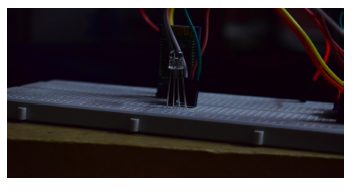
\includegraphics[width=\linewidth,height=8cm] {./images/p17.png}
	\caption{RGB LED}
	\label{manual}
\end{figure}

\begin{figure}[H]
	
	\centering
	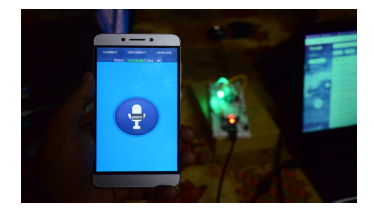
\includegraphics[width=\linewidth,height=8cm] {./images/p18.png}
	\caption{Test Case-I}
	\label{manual}
\end{figure}

\begin{figure}[H]
	
	\centering
	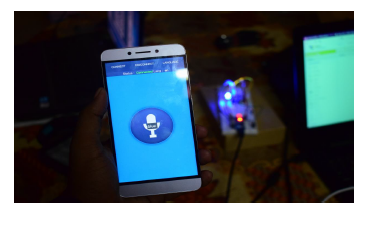
\includegraphics[width=\linewidth,height=8cm] {./images/p19.png}
	\caption{Test Case-II}
	\label{manual}
\end{figure}\\

iHALO Voice APP
\begin{figure}[H]
	
	\centering
	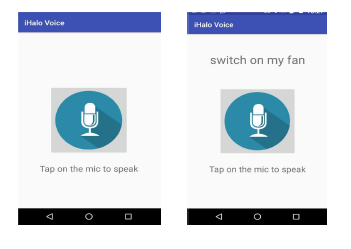
\includegraphics[width=\linewidth,height=8cm] {./images/p20.png}
	\caption{iHALO Voice App}
	\label{manual}
\end{figure}\\

AR APP
\begin{figure}[H]
	
	\centering
	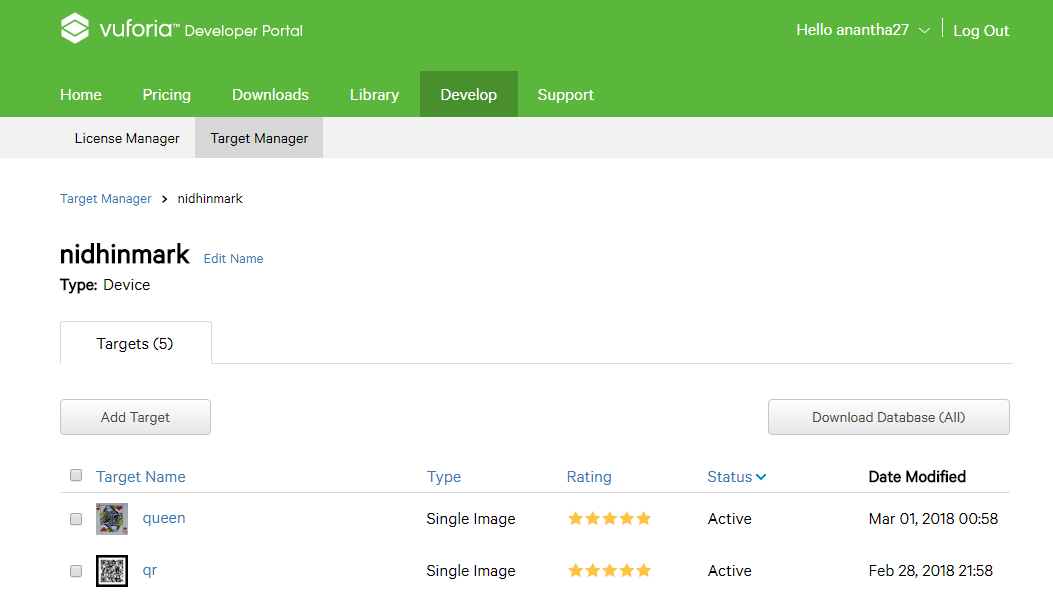
\includegraphics[width=\linewidth,height=9cm] {./images/p21.png}
	\caption{Vuforia SDK}
	\label{manual}
\end{figure}\\


\begin{figure}[H]
	
	\centering
	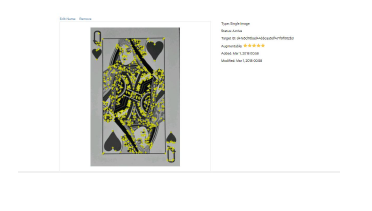
\includegraphics[width=\linewidth,height=7cm] {./images/p25.png}
	\caption{Image Processing}
	\label{manual}
\end{figure}\\


\begin{figure}[H]
	
	\centering
	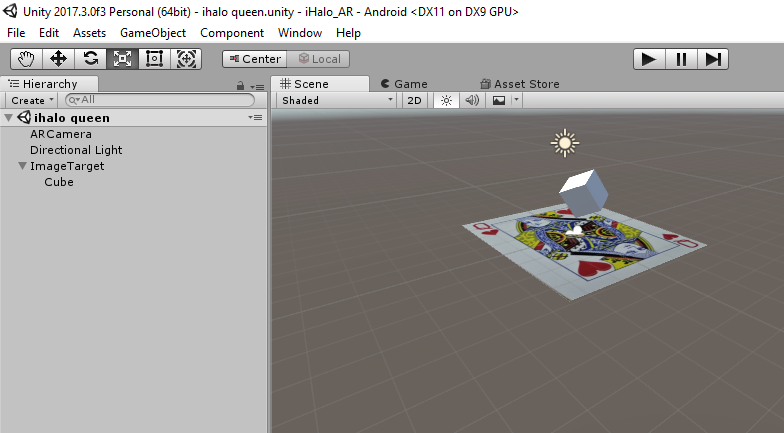
\includegraphics[width=\linewidth,height=9cm] {./images/p26.png}
	\caption{Unity 3D Development}
	\label{manual}
\end{figure}

\begin{figure}[H]
	
	\centering
	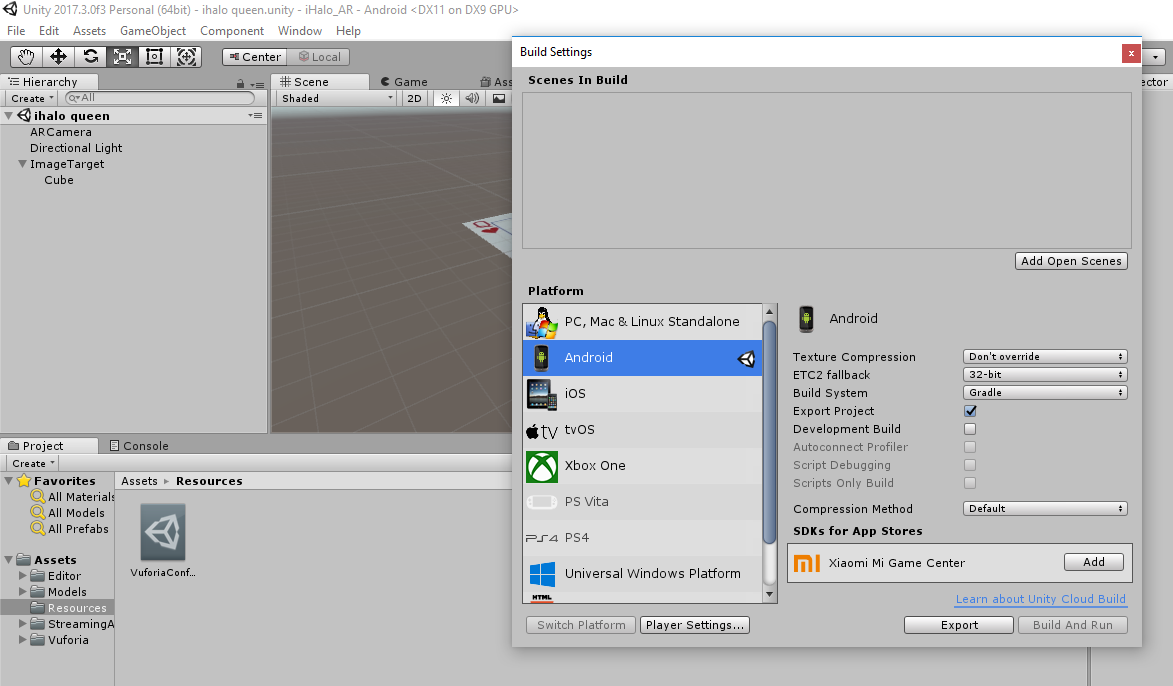
\includegraphics[width=\linewidth,height=8cm] {./images/p27.png}
	\caption{Exporting the Project}
	\label{manual}
\end{figure}

\section{Appendix-III: Output}
\begin{figure}[H]
	
	\centering
	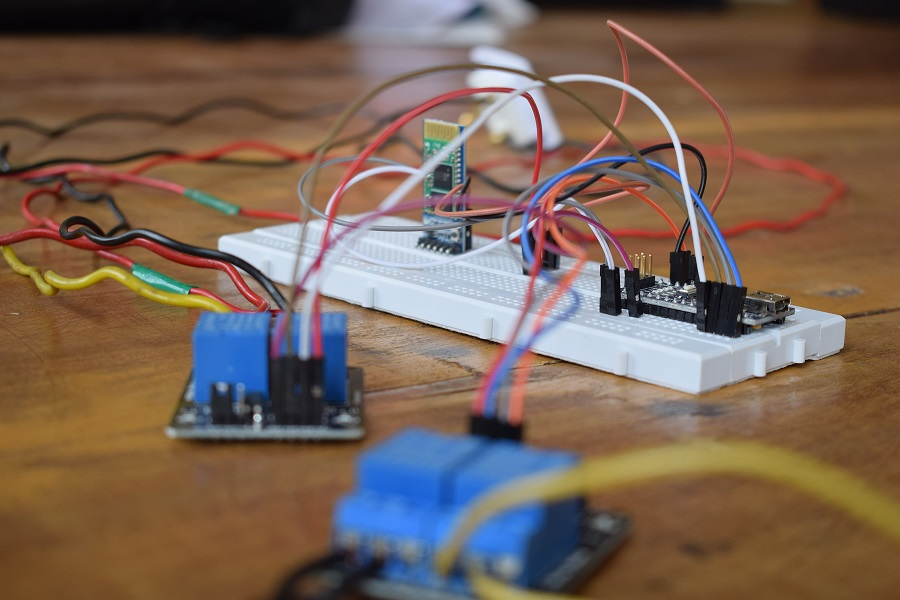
\includegraphics[width=\linewidth,height=9cm] {./images/p28.jpg}
	\caption{Output Setup}
	\label{manual}
\end{figure}

\begin{figure}[H]
	
	\centering
	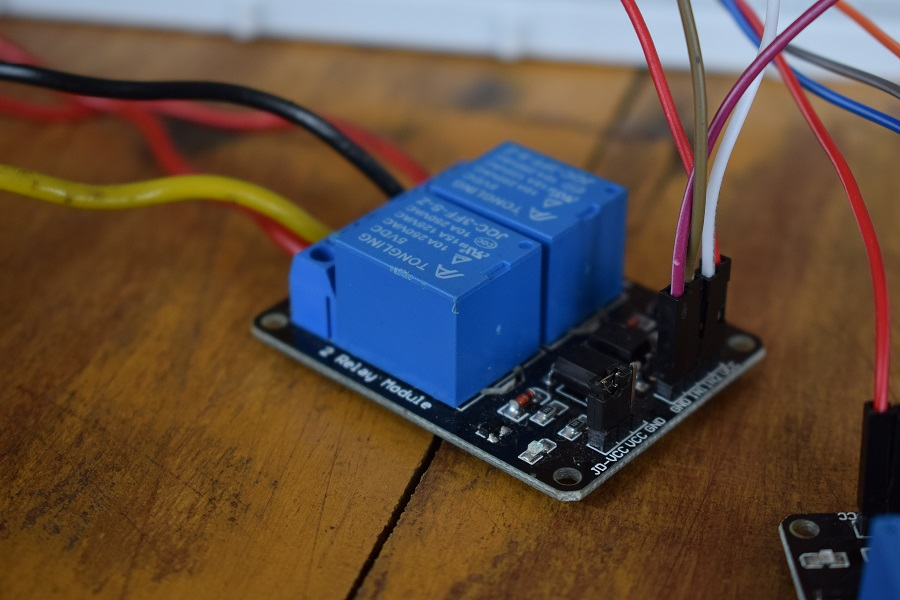
\includegraphics[width=\linewidth,height=9cm] {./images/p29.jpg}
	\caption{Relay Module-Input}
	\label{manual}
\end{figure}

\begin{figure}[H]
	
	\centering
	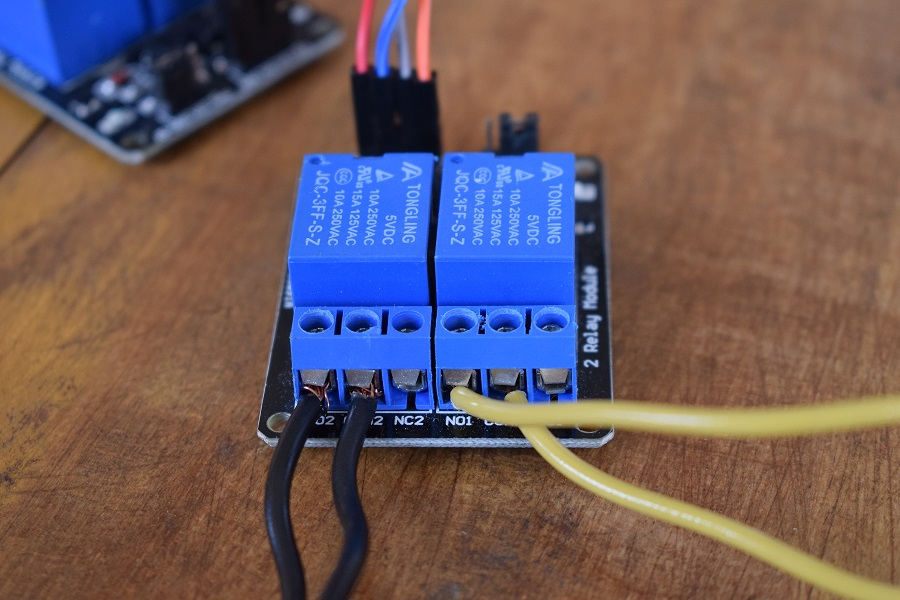
\includegraphics[width=\linewidth,height=9cm] {./images/p30.jpg}
	\caption{Relay Module-Output}
	\label{manual}
\end{figure}

\begin{figure}[H]
	
	\centering
	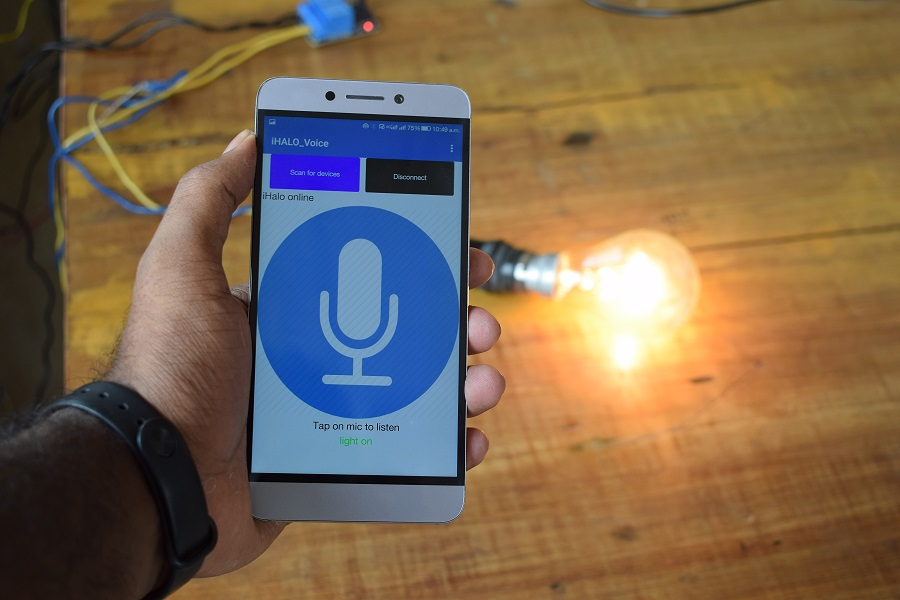
\includegraphics[width=\linewidth,height=9cm] {./images/p31.jpg}
	\caption{Test Case-III}
	\label{manual}
\end{figure}

\begin{figure}[H]
	
	\centering
	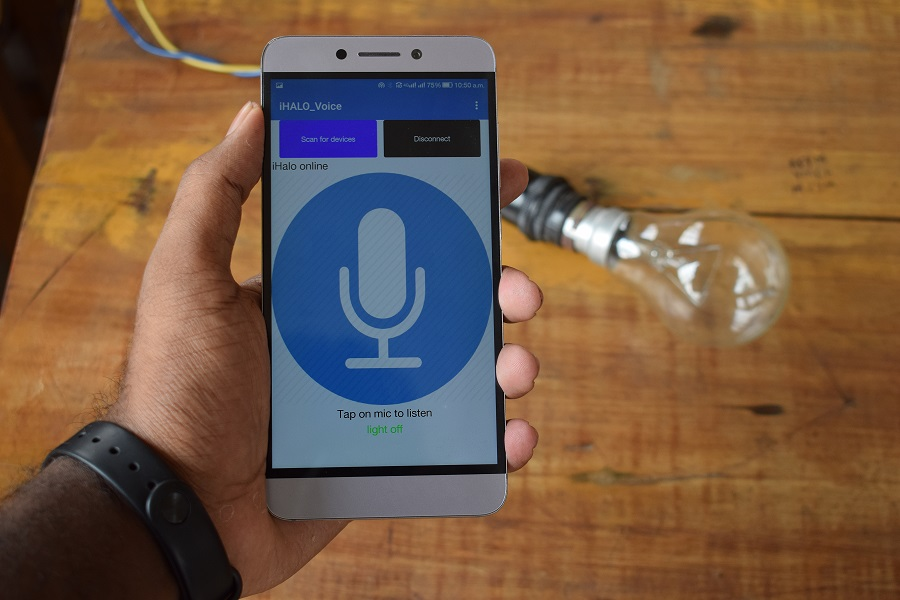
\includegraphics[width=\linewidth,height=9cm] {./images/p32.jpg}
	\caption{Test Case-IV}
	\label{manual}
\end{figure}

\begin{figure}[H]
	
	\centering
	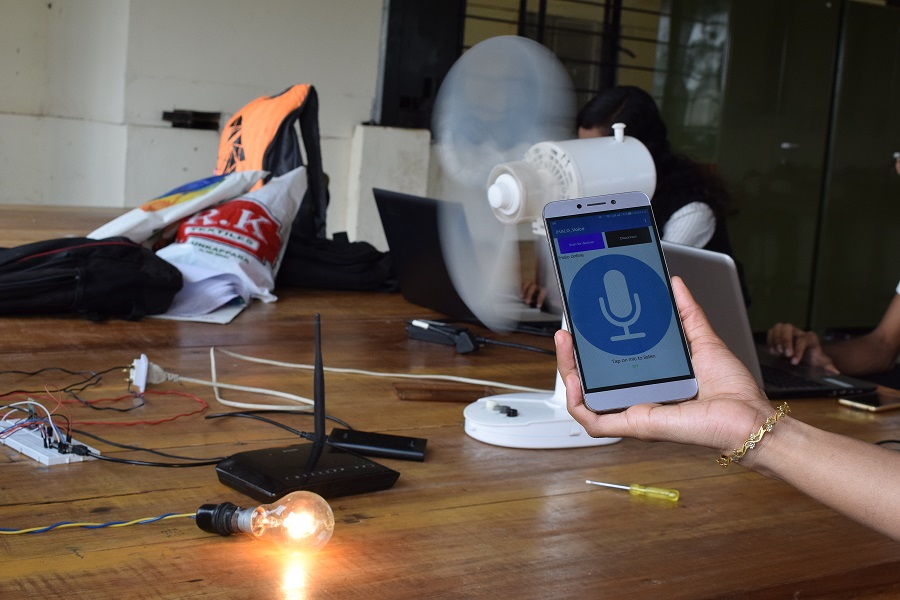
\includegraphics[width=\linewidth,height=9cm] {./images/p33.jpg}
	\caption{Test Case-V}
	\label{manual}
\end{figure}

\begin{figure}[H]
	
	\centering
	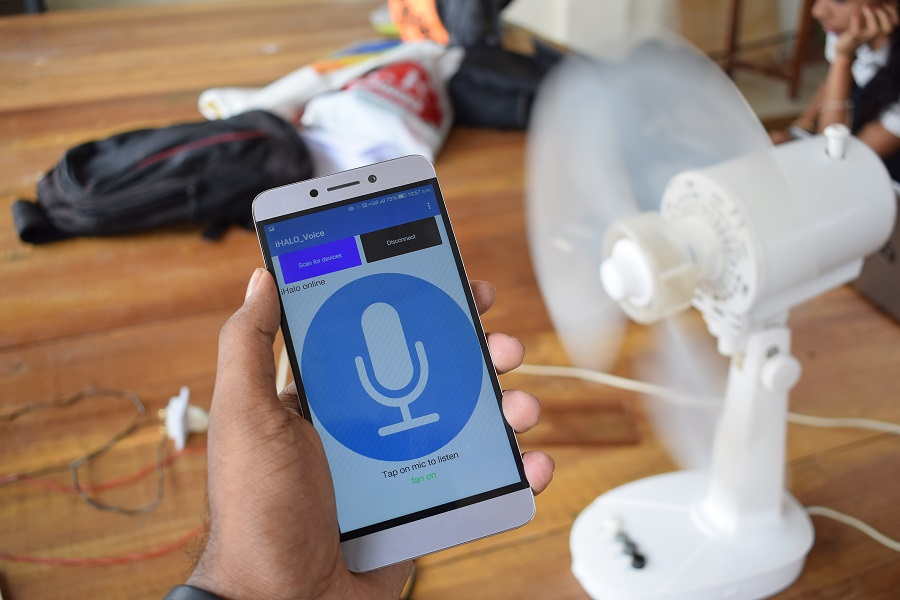
\includegraphics[width=\linewidth,height=9cm] {./images/p34.jpg}
	\caption{Test Case-VI}
	\label{manual}
\end{figure}

\begin{figure}[H]
	
	\centering
	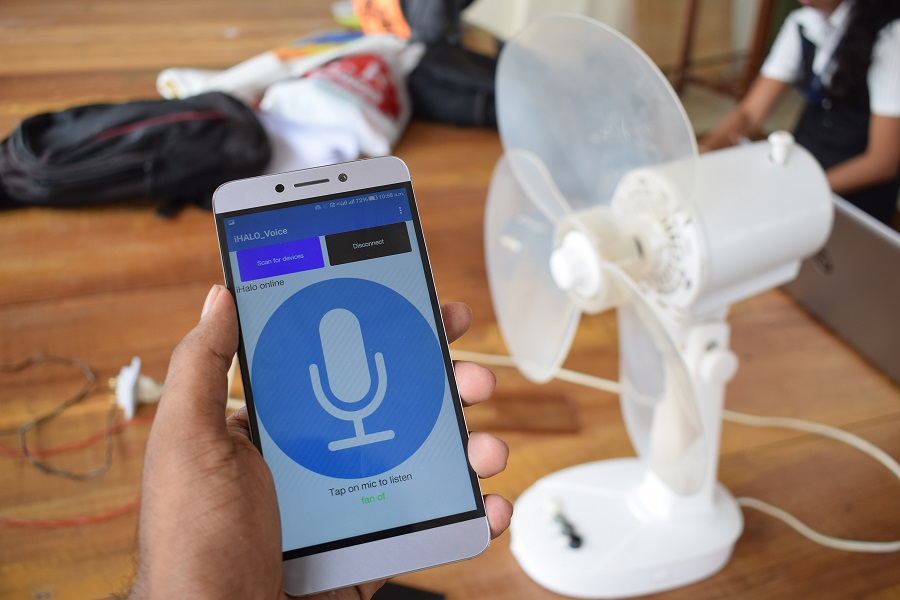
\includegraphics[width=\linewidth,height=9cm] {./images/p35.jpg}
	\caption{Test Case-VII}
	\label{manual}
\end{figure}

\begin{figure}[H]
	
	\centering
	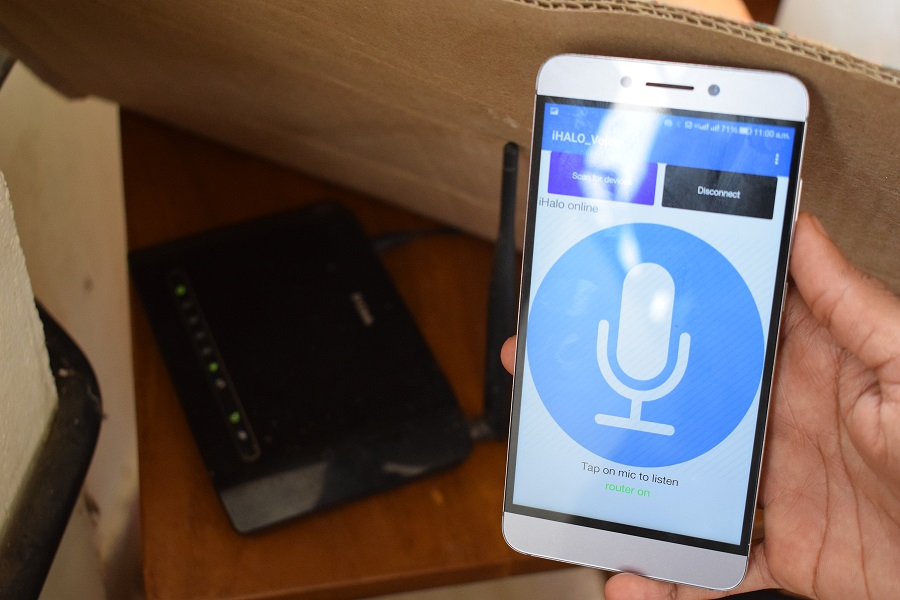
\includegraphics[width=\linewidth,height=9cm] {./images/p36.jpg}
	\caption{Test Case-VIII}
	\label{manual}
\end{figure}

\begin{figure}[H]
	
	\centering
	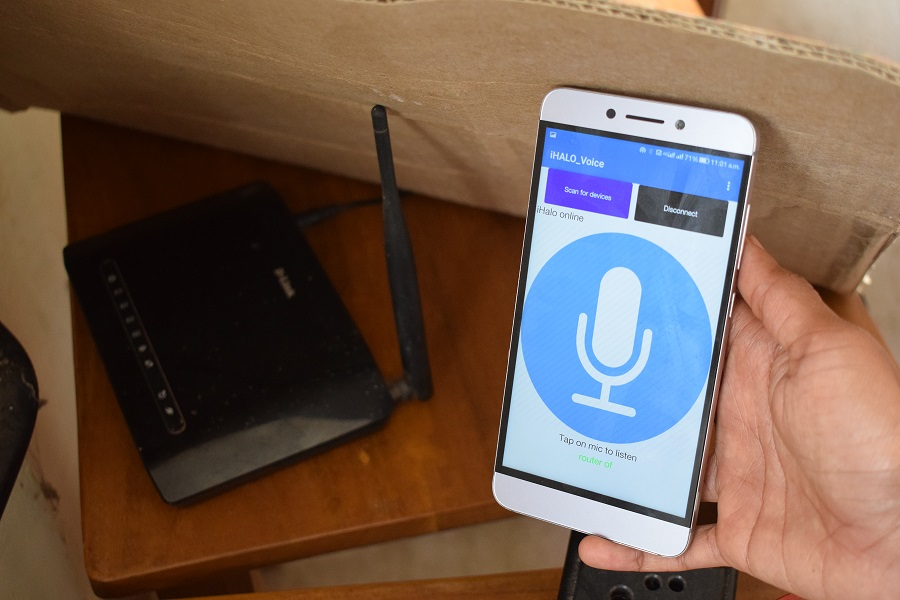
\includegraphics[width=\linewidth,height=9cm] {./images/p37.jpg}
	\caption{Test Case-IX}
	\label{manual}
\end{figure}

\begin{figure}[H]
	
	\centering
	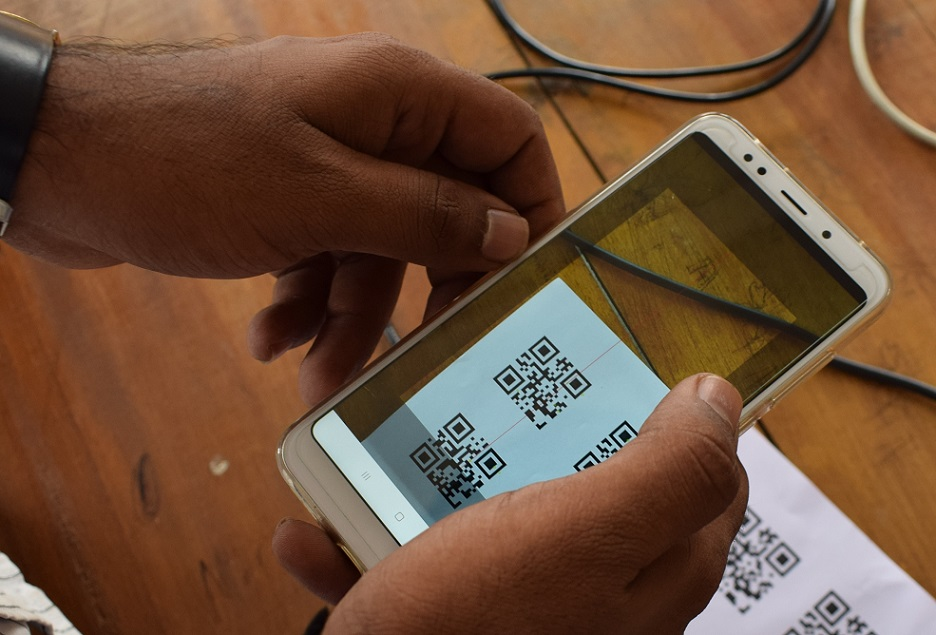
\includegraphics[width=\linewidth,height=9cm] {./images/p38.jpg}
	\caption{AR Scanning}
	\label{manual}
\end{figure}

\begin{figure}[H]
	
	\centering
	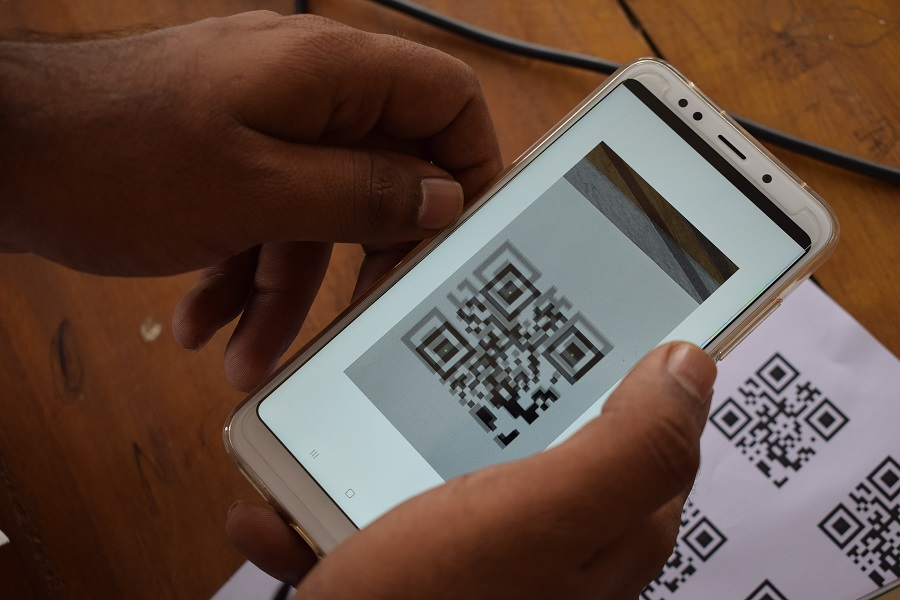
\includegraphics[width=\linewidth,height=9cm] {./images/p39.jpg}
	\caption{AR Detection}
	\label{manual}
\end{figure}

\begin{figure}[H]
	
	\centering
	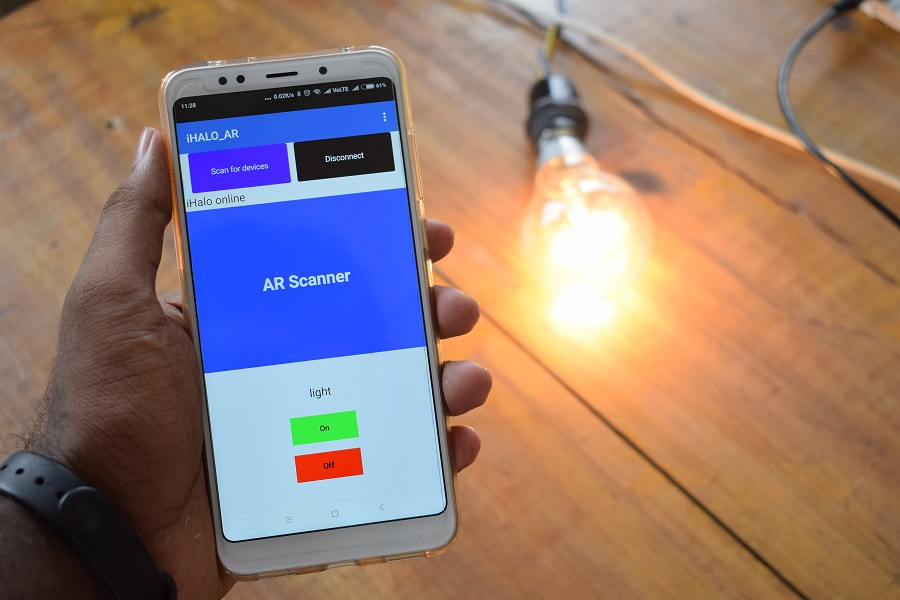
\includegraphics[width=\linewidth,height=9cm] {./images/p40.jpg}
	\caption{AR App}
	\label{manual}
\end{figure}

\begin{figure}[H]
	
	\centering
	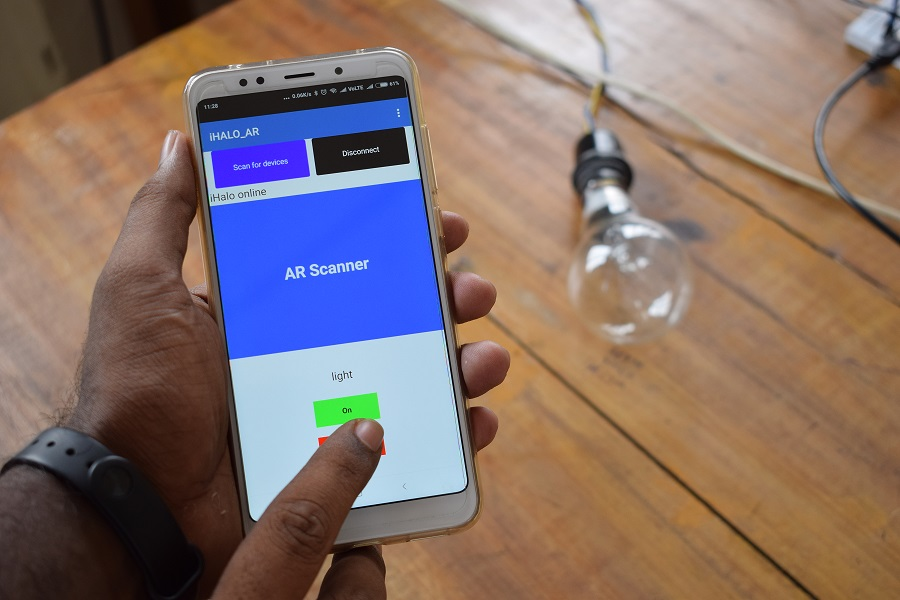
\includegraphics[width=\linewidth,height=9cm] {./images/p41.jpg}
	\caption{Test Case-X}
	\label{manual}
\end{figure}

\begin{figure}[H]
	
	\centering
	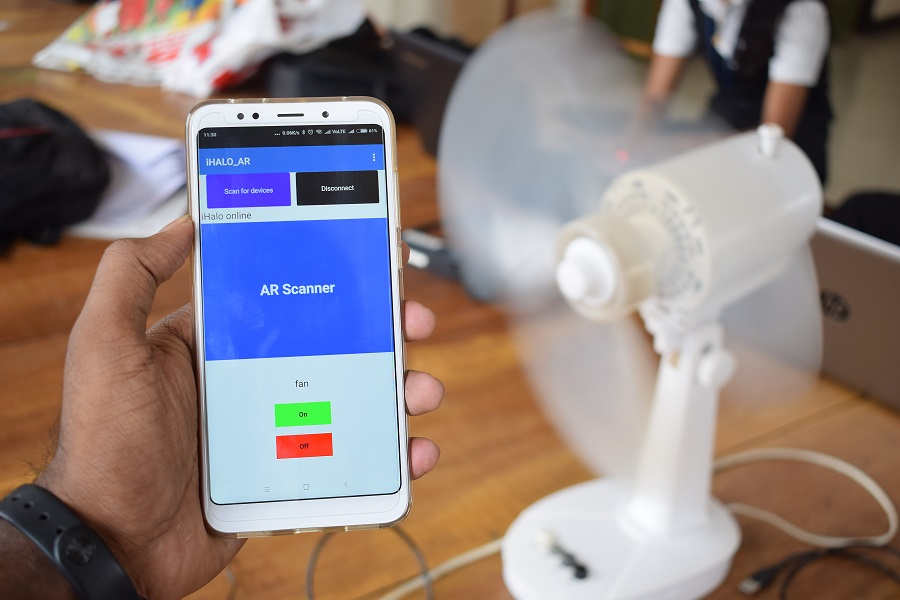
\includegraphics[width=\linewidth,height=9cm] {./images/p42.jpg}
	\caption{Test Case-XI}
	\label{manual}
\end{figure}

\begin{figure}[H]
	
	\centering
	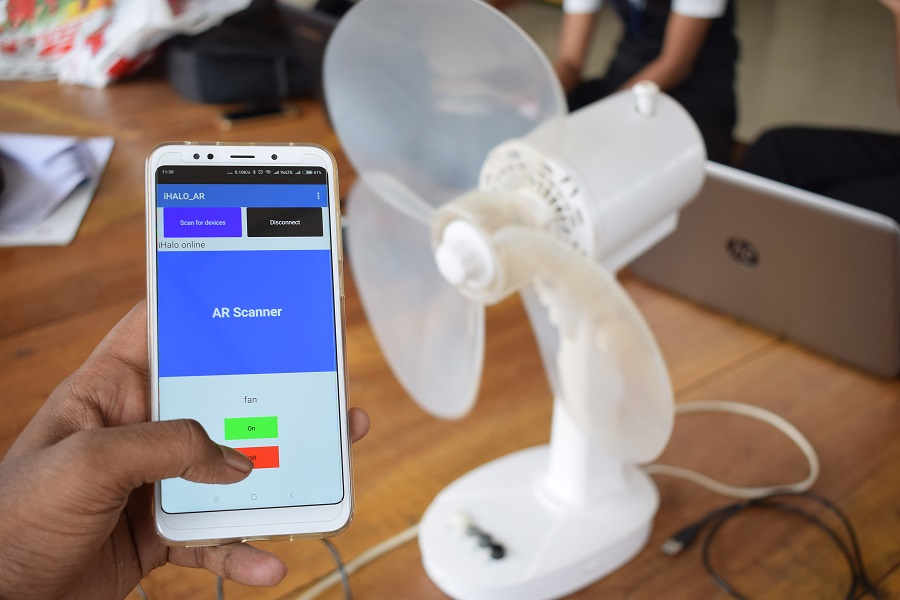
\includegraphics[width=\linewidth,height=9cm] {./images/p43.jpg}
	\caption{Test Case-XIII}
	\label{manual}
\end{figure}

\chapter{Conclusion}
\thispagestyle{fancy}
iHALO is an android based home automation system which makes the system more flexible and attractive user interface compared to other home automation systems. Using a simple android app we can control electrical appliances with voice commands or with the help of Augmented Reality. So there is no need for you to get up to switch on or switch off the device while watching a movie or doing some important work. The system comprises of a Wifi module, Arduino board and relay modules. Wifi module is used as the communication channel between android phone and the Arduino Board.

\chapter{Future Scope}
\thispagestyle{fancy}
We are planning to implementing low power Wi-Fi module would be better. Improving our system to report power use of each appliance. Implementing light weight protocol like MQTT would be better. Use of Node Js can decrease our waiting time of response. Our wish is to implement our project in all the possible situation like in offices, industries, schools, cars etc. As we already see there are lots of issues in previous existing approaches. In this section we present primarily focusing on, the use of loT for the advance, energy efficient and selflearning home automation system. The main objective is to design and implement cost effective and smart home automated system. We are using Wi-Fi based approach for communication between Server and Home appliances. This smart home automated system will design with the implementation of related software and hardware. The project proposes an implementation of IoT (Internet of Things) based smart home automated system for remotely control the home appliances using Wi-Fi. Low cost Wi-Fi module ESP8266 is used to build Smart Units. The user will operate home appliances like lights; fans are remotely controlled through Android App. The server will be interfaced with relay hardware circuits that control the appliances running at home.

\chapter{References}
\thispagestyle{fancy}
1. Specialization on Internet of things.[Online]\\
2. Android App Development.[Online]\\
3. Augmented Reality App Development.[Online]\\
4. Blynk Platform for IoT.[Online]\\
5. Fundamentals of software engineering by Rajib mall, PHI Learning.\\